\documentclass[compress]{beamer}

\usepackage[utf8]{inputenc}
\usepackage{graphicx}
\usepackage{color}
\usepackage{colortbl}
\usepackage{listings}
\usepackage{caption}
\usepackage{pgfpages}
\usepackage{tabularx}
\usepackage{amsthm}
\usepackage{url}

%\usetheme[basergb={1,0.2,0.2}]{Dcon}
%\usetheme[baseRGB={23,102,34}]{Dcon}
\usetheme{Dcon} % default color

%%%%%%%%%%%%%%%%%%%%%%%%%%%%% Definitions %%%%%%%%%%%%%%%%%%%%%%%%%%%%%%%%%%%%%

\newcommand{\logounis}{
\begin{table}[h]
\centering
\begin{tabular}{ccc}

\includegraphics[width=.3\linewidth]{images/logos/lmu_logo} \hspace{0.3cm} &

\includegraphics[width=.3\linewidth]{images/logos/Uni_Aug_Logo_Basis_pos_A}
\hspace{0.3cm} &

\includegraphics[width=.3\linewidth]{images/logos/tum}
\end{tabular}
\end{table}}

\newcommand{\logose}{
\includegraphics[width=.2\linewidth]{images/logos/LogoSEengl}\hspace{5mm}}

\newcommand{\hl}[1]{\fcolorbox{red}{white}{#1}}
\newcommand{\todo}[1]{\hl{TODO: #1...}}
\newcommand{\review}[0]{\todo{REVIEW}}
\newcommand{\comm}[1]{\textsuperscript{\bf \color{red}{\tiny [#1]}}}
\newcommand{\q}[0]{\comm{?}}
\newcommand{\s}[0]{\comm{*}}

\newcommand{\scite}[1]{\textsuperscript{\tiny\cite{#1}}}

%\bibliographystyle{apalike}


\titlegraphic{\logounis}
\title[Visual Debugging for Robotics]
{A flexible visual framework\\ \strut for debugging complex robotic systems}
\subtitle{\scriptsize{Masters's Thesis in the Software Engineering Elite Graduate Program}}
\author[Felix Kaser]{Felix Kaser\\\tiny{\texttt{kaserf@in.tum.de}}}
%\institute[ISSE]
%{Institut für Software \& Systems \\
%Engineering}
\date{October 3, 2012}

\logo{\logose}

\additionaltext{\tiny
{Supervisors: Prof. Dr. Wolfgang Reif,\\
\hspace{20mm}Prof. Bruce A.~MacDonald, PhD.\\
\hspace{2mm}Advisor: M.Sc. Andreas Angerer}}

%%%%%%%%%%%%%%%%%%%%%%%%%%%%% Document %%%%%%%%%%%%%%%%%%%%%%%%%%%%%%%%%%%%%%%%%

\begin{document}

% title page
\begin{frame}[plain]
\titlepage
\end{frame}

\begin{frame}{Outline}
\tableofcontents
\end{frame}

\section{Introduction}
%%%%%%%%%%%%%%% Introduction %%%%%%%%%%%%%%%%%%%%%%%
\subsection{Problem Statement}

\begin{frame}{Problem Statement}
\begin{itemize}
\item Debugging in robotics is complex
\item Traditional debugging tools lack support for robotics
\item Specialized tools are needed to cope with the requirements of robotics
\end{itemize}
\pause
\textbf{Key problems:}
\begin{itemize}
\item Robotic applications are usually not interruptible
\item The data handled in robotic systems comes from sensors instead of user-input
\item Data is hard to understand in its raw form
\item The robotics field is diverse and tools are often created for really specific use cases and cannot be easily re-used
\end{itemize}
\end{frame}

\begin{frame}{Hypothesis}
\begin{block}{}
A visualization tool for robotics that allows developers to choose the visualization they prefer can reduce the cognitive load during debugging and thus improve development speed.
\end{block}
\end{frame}

\subsection{Debugging in Robotics}

\begin{frame}{Related Tools}
\begin{itemize}
\item Realtime Debugging \cite{Gumbley2009}
\item National Instruments LabVIEW
\item Augmented Reality (AR) Debugging \cite{Collett2010}
\end{itemize}
\end{frame}

\begin{frame}{Realtime Debugging}
\begin{columns}
\begin{column}{.5\textwidth}
\begin{itemize}
\item Developed by Luke Gumbley at the robotics lab
\item Extends GDB to support realtime data collection
\item Integrated into NetBeans IDE
\end{itemize}
\end{column}
\hfill%
\begin{column}{.5\textwidth}
\begin{figure}[htbp]
  \centering
  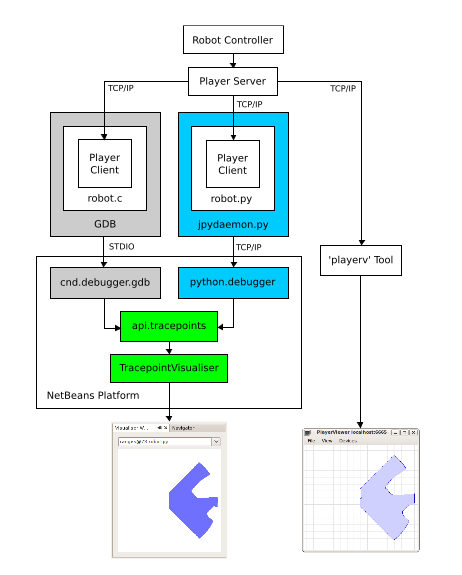
\includegraphics[width=.75\textwidth]{images/tracepoints_gumbley.png}
  \caption{Tracepoints block diagram. \cite{Gumbley2009}}
\end{figure}
\end{column}
\end{columns}
\end{frame}

\begin{frame}{LabVIEW}
\begin{itemize}
\item Graphical programming tool developed by National Instruments
\item Front panels allow to create specific user interfaces for the program
\item Front panels are connected in the visual program
\end{itemize}
\end{frame}

\begin{frame}{LabVIEW}
% source: public domain image from http://en.wikipedia.org/wiki/File:WikipediaFPandBD.png
\begin{figure}[htbp]
  \centering
  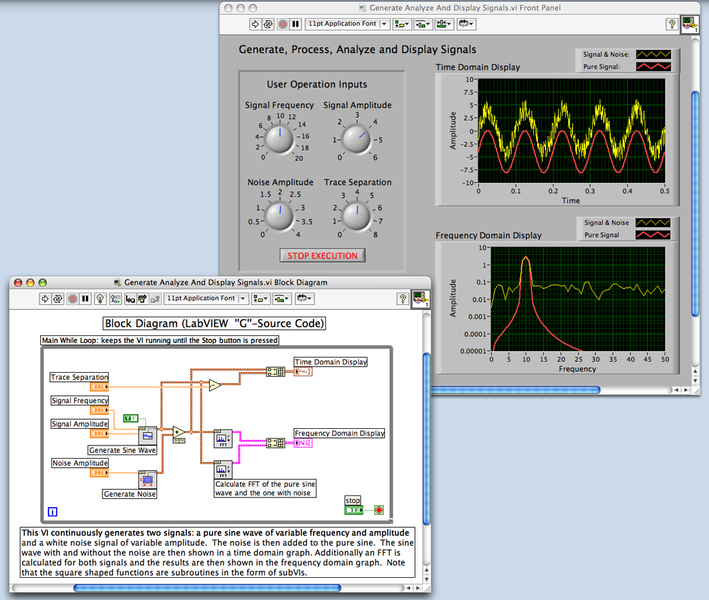
\includegraphics[width=.6\textwidth]{images/labview_frontpanel.png}
  \caption{Screenshot of the LabVIEW user interface with front panels in the top right.}
\end{figure}
\end{frame}

\begin{frame}{AR Dev Framework}
\begin{itemize}
\item Developed by Toby Collett at the robotics lab
\item Augmented reality visualizations
\item Helps to understand how the robot perceives the environment
\item Relies on a (complicated) tracking setup
\end{itemize}
\end{frame}

\begin{frame}{AR Dev Framework}
\begin{figure}[htbp]
  \centering
  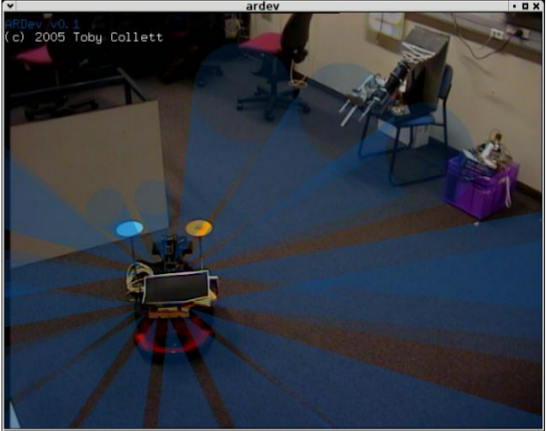
\includegraphics[width=.6\textwidth]{images/ar_view.png}
  \caption{Screenshot of augmented reality view. \cite{Collett2007}}
\end{figure}
\end{frame}

\begin{frame}{Problems of Existing Tools}
\begin{itemize}
\item High configuration overhead
\item Visualization focuses on pre defined data
\item Arbitrary data is usually rendered as text
\item Lack of transparency
\end{itemize}
\end{frame}

\section{ROS (Robot Operating System)}

\subsection{Overview}

\begin{frame}
\begin{figure}[htbp]
  \centering
  
\includegraphics[width=.4\textwidth]{images/ros_logo.png}
  %\caption{Screenshot of augmented reality view. \cite{Collett2007}}
\end{figure}
\end{frame}

\begin{frame}{Overview}

\begin{columns}
\begin{column}{.6\textwidth}
%left column
\begin{itemize}
\item Developed first at Stanford, now at Willow Garage
\item Modular robotic middleware
\item Active open source community
\item Many ready to use solutions for common problems in robotics (SLAM, joint transformations, grasping, ...)
\end{itemize}
\end{column}%
\hfill%
\begin{column}{.48\textwidth}
%right column
\begin{figure}[t]
    \centering
    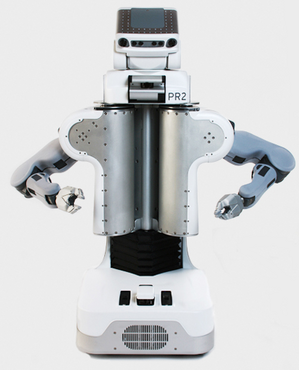
\includegraphics[width=0.7\textwidth]{images/pr2.png}
    \caption[The PR2 robot]{The PR2 robot}
\end{figure}
\end{column}%
\end{columns}
\end{frame}

%\subsection{ROS Basics}
\begin{frame}{ROS Basics}
\begin{itemize}
\item Modules are called nodes
\item Communication infrastructure based on publish/subscribe and services
\end{itemize}
\end{frame}

\begin{frame}{Publish Subscribe Mechanism}
\begin{figure}[t]
    \centering
    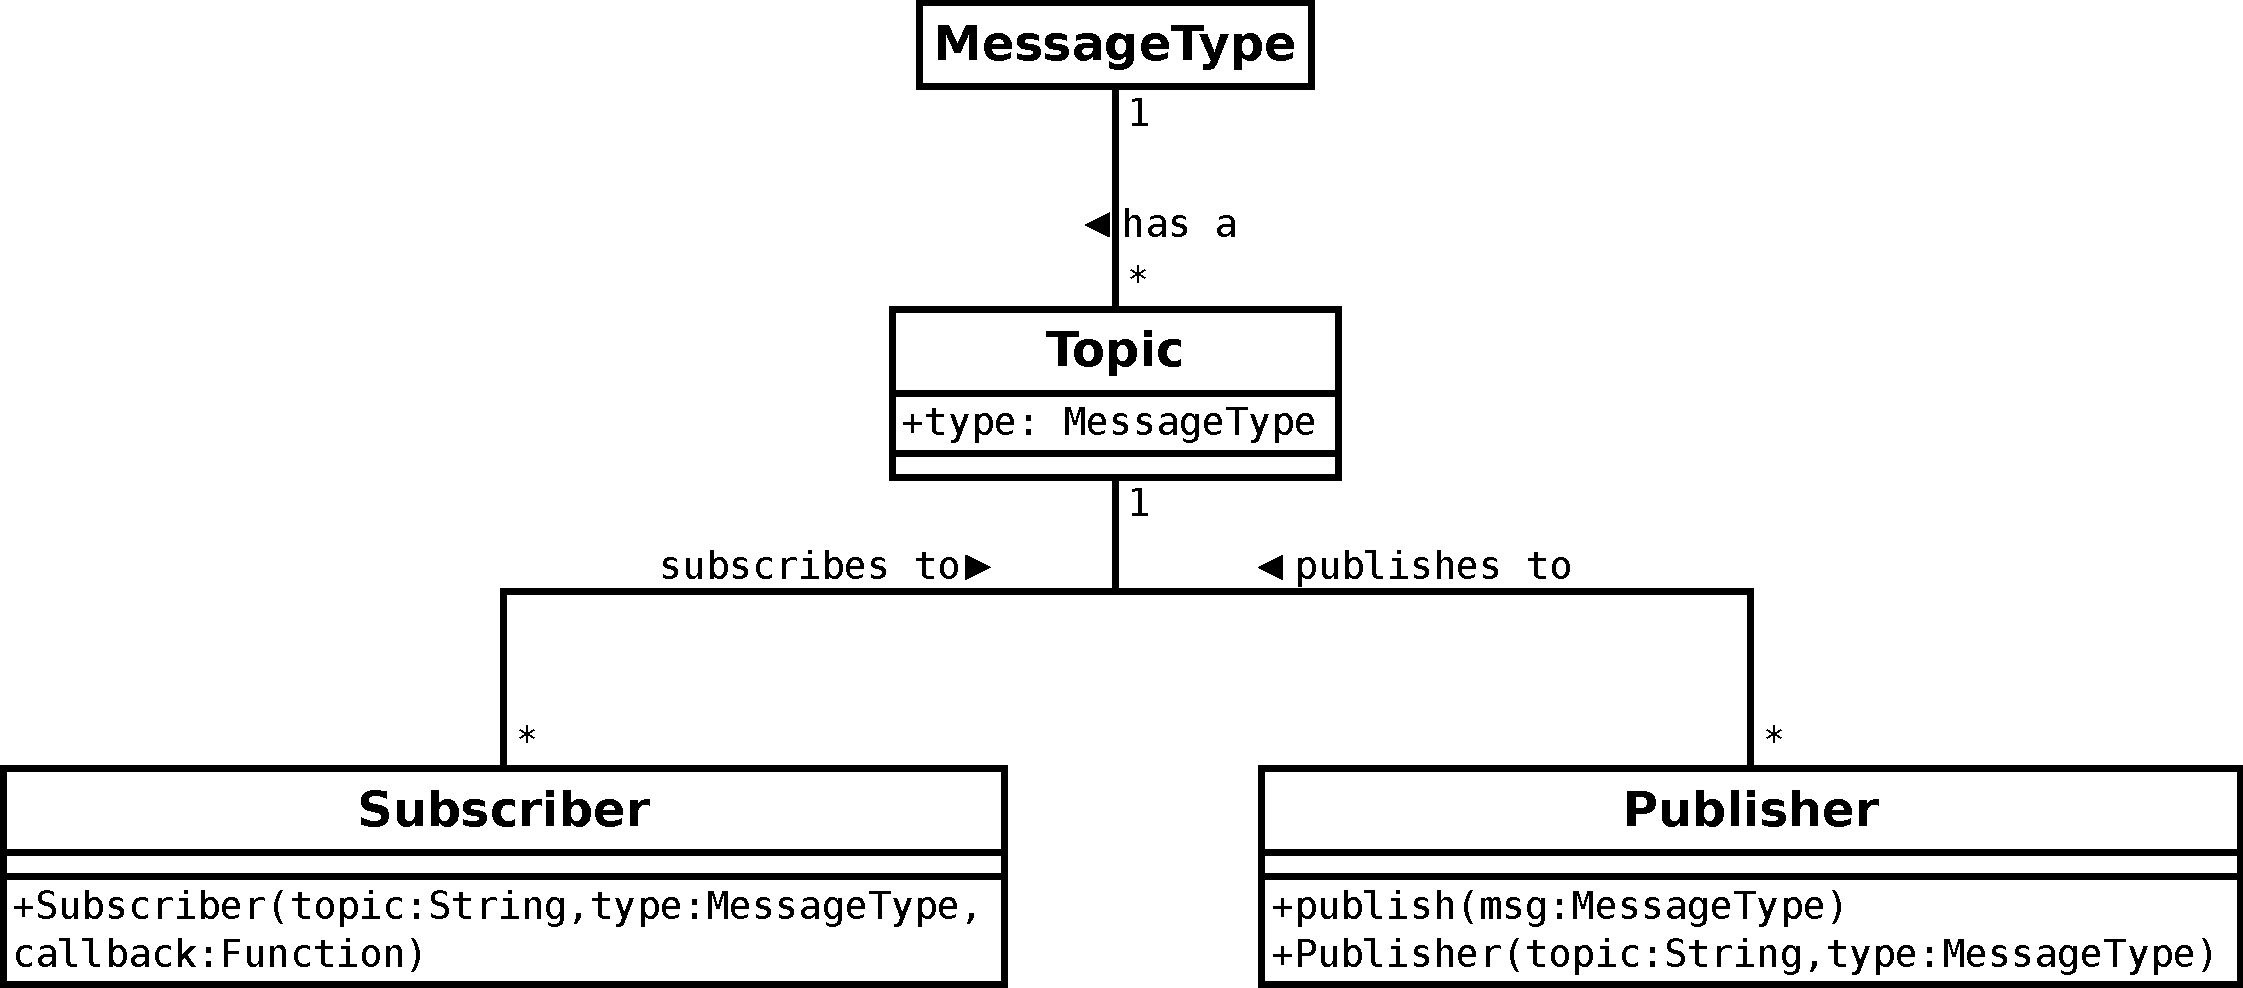
\includegraphics[width=\textwidth]{diagrams/ros_pubsub}
\end{figure}
\end{frame}

\begin{frame}{Publish Subscribe Summary}
\begin{itemize}
\item Popular message passing method for push messages
\item Flexible regarding the network topology: routing happens during runtime
\item Decouples sender from receiver (loose coupling)
\item Does not guarantee delivery
\item Is used in ROS to communicate between nodes
\end{itemize}
\end{frame}

\subsection{Existing ROS Tools}
\begin{frame}{Existing ROS Tools}

\begin{columns}
\begin{column}{.4\textwidth}
%first column
\begin{figure}[t]
    \centering
    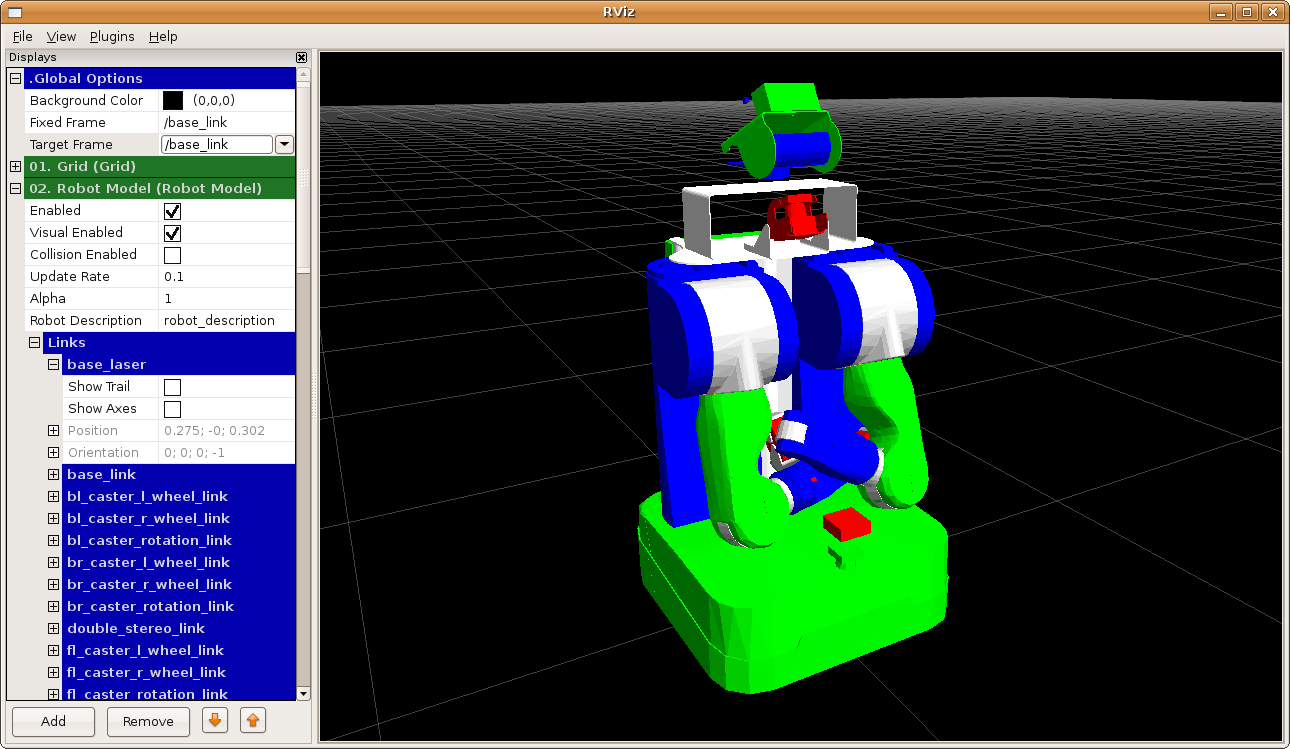
\includegraphics[width=.9\textwidth]{images/RVizRobotModel.png}
    \caption{RViz}
\end{figure}
\end{column}%
\hfill%
\begin{column}{.4\textwidth}
%second column
\begin{figure}[t]
    \centering
    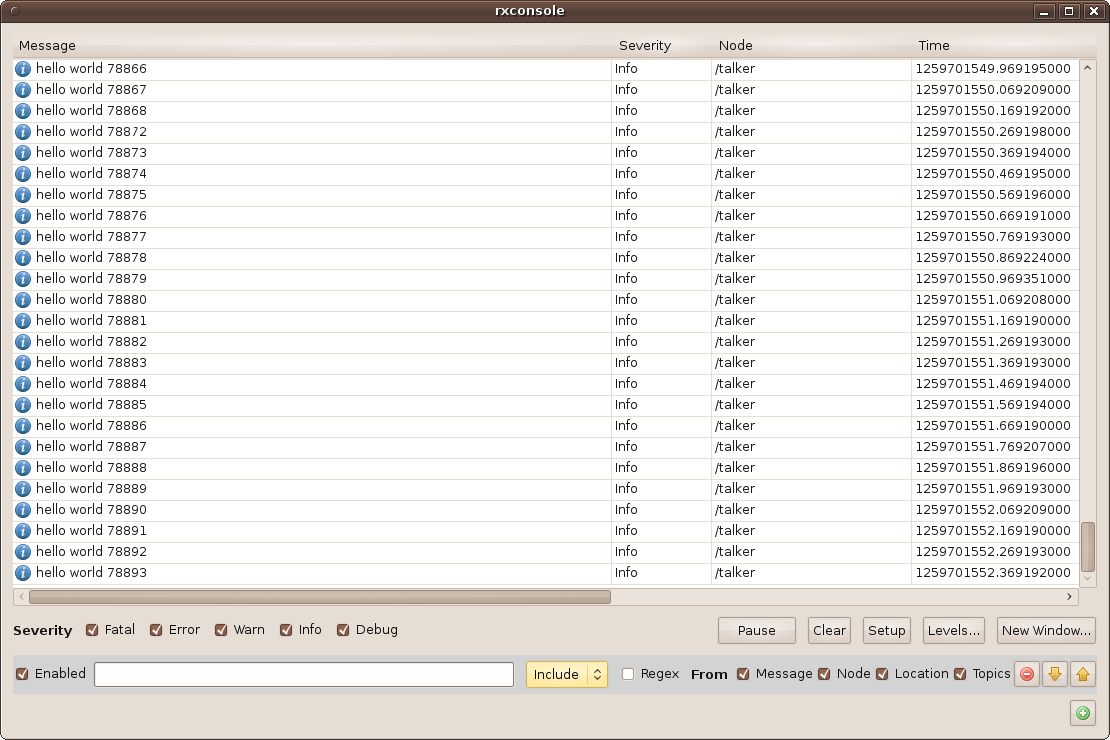
\includegraphics[width=.9\textwidth]{images/rxconsole.png}
    \caption{rxconsole}
\end{figure}
\end{column}%
\hfill%
\begin{column}{.4\textwidth}
%third column
\begin{figure}[t]
    \centering
    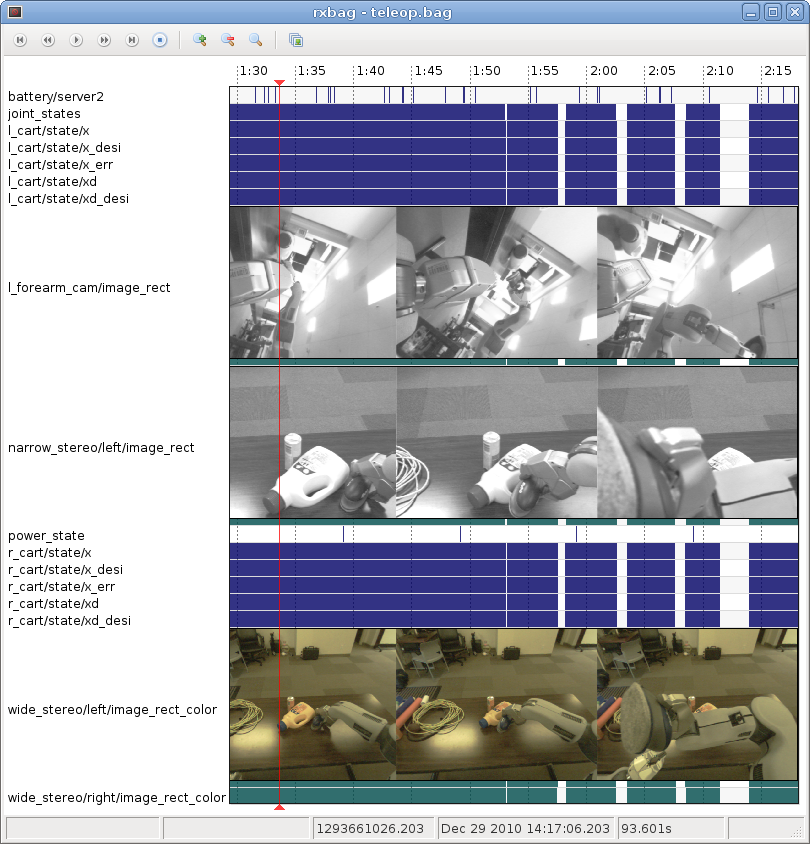
\includegraphics[width=.85\textwidth]{images/rxbag_screenshot.png}
    \caption{rxbag}
\end{figure}
\end{column}
\end{columns}
\end{frame}

%\subsection{Logging in ROS}
\begin{frame}{Logging in ROS}
\begin{itemize}
\item C++ and Python client libraries contain logging API
\item Log messages are sent to console, log file and \emph{/rosout}
\item Can be filtered by severity and text
\item Log messages are text only with metadata (timestamp)
\end{itemize}
\end{frame}

\section{ROSDashboard}
%%%%%%%%%%%%%%%% ROSDashboard section %%%%%%%%%%%%%%%%%%%
\subsection{Goals}

\begin{frame}{ROSDashboard}
\begin{figure}[t]
    \centering
    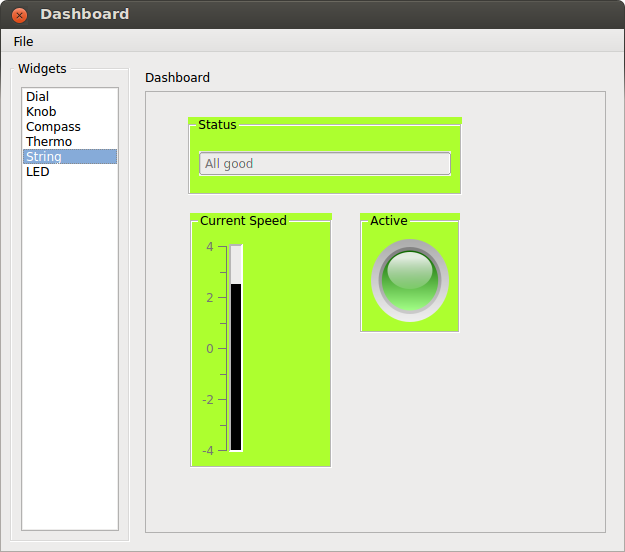
\includegraphics[height=.7\textheight]{images/rosdashboard_screenshot.png}
\end{figure}
\end{frame}

\begin{frame}{Goals}
\begin{itemize}
\item Create a easy to use debugging tool
\item Visualize simple and abstract data
\item Allow developers to choose the visualization they prefer
\item Extendible through plugins
\item Data collection inspired by logging statements
\item Create a tool to evaluate hypothesis
\end{itemize}
\end{frame}

\subsection{Requirements}
\begin{frame}{Requirements}
\begin{itemize}
\item Distributed \& live debugging
\item Transparently connect visualization to data
\item Adaptability to different preferences and use cases
\item Low configuration overhead to keep developer on task
\end{itemize}
\end{frame}

\subsection{Design}

\begin{frame}{System Design}
\begin{itemize}
\item Make use of ROS topics for transparent access to data
\item Flexible and configurable user interface dashboard
\item Wrap visualizations in widgets
\item Framework that allows easy integration of a plugin system
\end{itemize}
\end{frame}

\begin{frame}{System Design}
\begin{figure}[t]
    \centering
    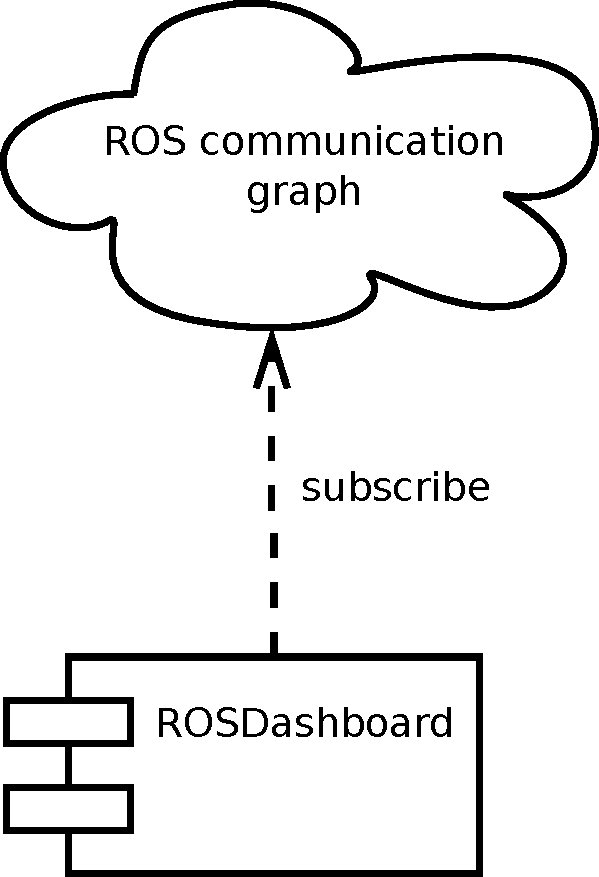
\includegraphics[height=.7\textheight]{diagrams/simple_architecture_overview}
		\caption{Simple architecture overview}
\end{figure}
\end{frame}

\begin{frame}{Object Design}
\begin{figure}
    \centering
    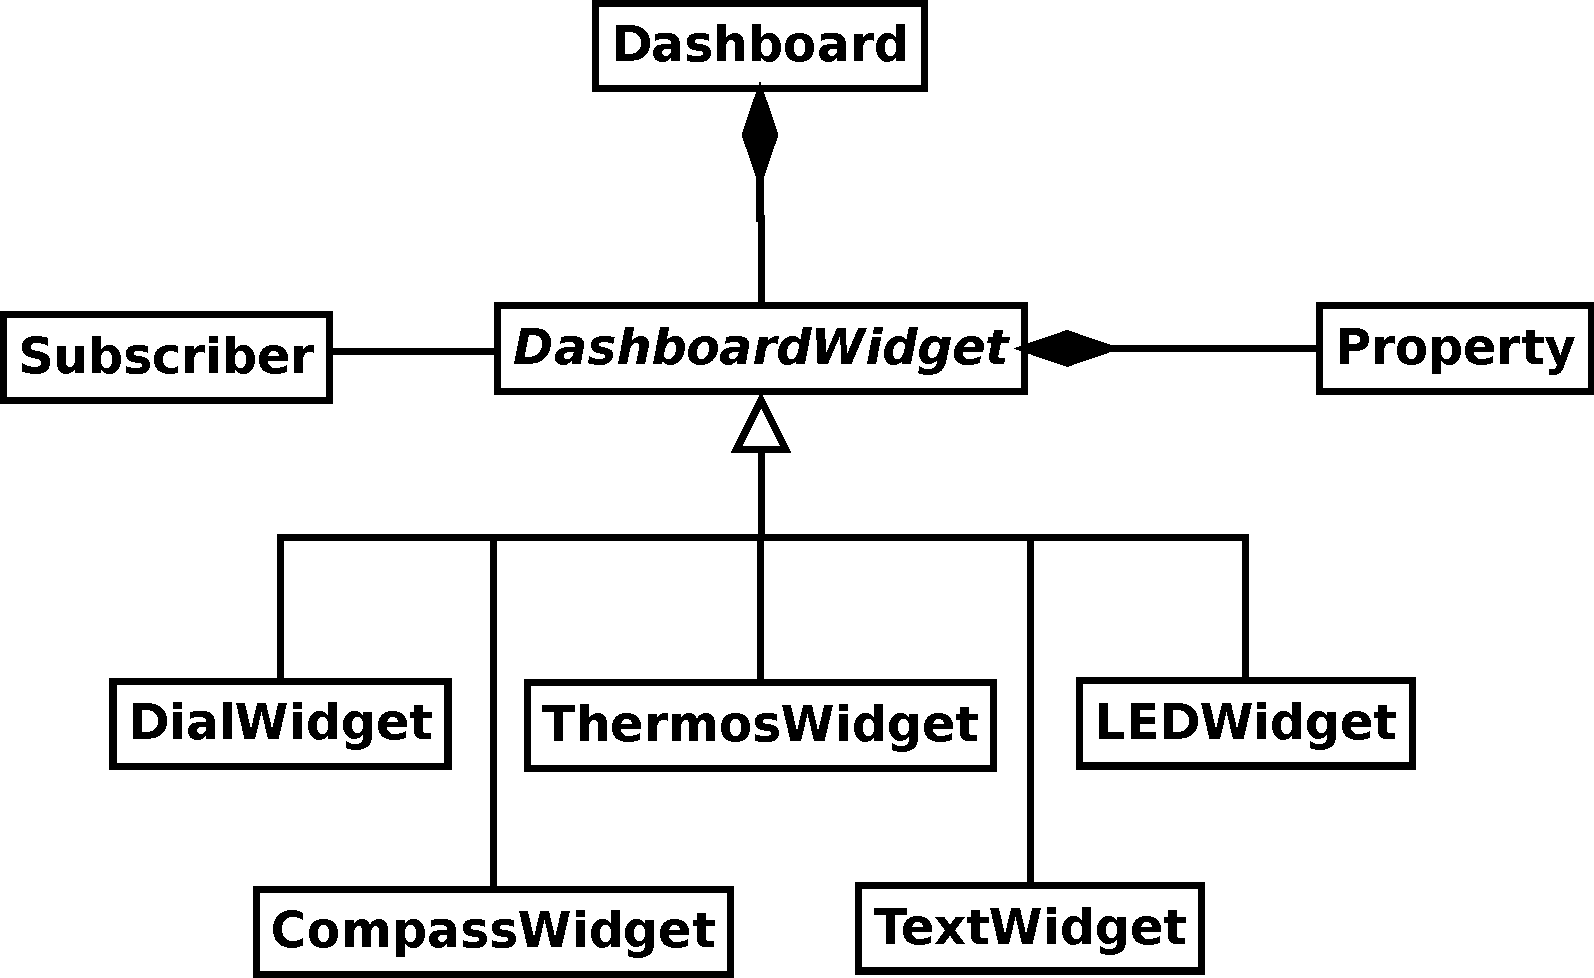
\includegraphics[width=0.7\textwidth]{diagrams/class_overview}
    \caption[Core object model overview]{Core object model overview}
\end{figure}
\end{frame}

\section{Outlook}

\subsection{Conclusion}

\begin{frame}{Conclusion}
\begin{itemize}
\item A flexible visual debugging system was designed
\item ROSDashboard has been implemented as a prototype of such a system
\item Minimal invasive data collection
\item It shows the potential of a flexible visualization tool for arbitrary data
\end{itemize}
\end{frame}

\subsection{Future Work}

\begin{frame}{Future Work}
\begin{itemize}
\item User interface improvements
\item Plugin framework
\item Parse existing string log messages with regular expressions
\item Publish debugging messages only if the ROS node was initialized as debugging node
\item Evaluate in real life project
\end{itemize}
\end{frame}

\subsection{Thanks}

\begin{frame}
\begin{center}
\huge
Thanks for everyone's help and support. It was a great time.
\end{center}
\end{frame}

\begin{frame}{Incentive:}
\begin{columns}
\begin{column}{.5\textwidth}
Munich
\begin{figure}[t]
    \centering
    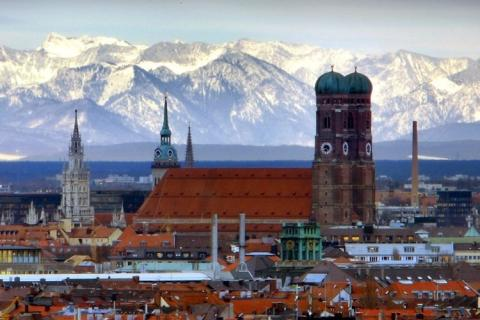
\includegraphics[width=.9\textwidth]{images/munich.jpg}
\end{figure}
\end{column}
\begin{column}{.5\textwidth}
South Tyrol\\
\tiny{(German speaking part of Italy ;) )}
\begin{figure}[t]
    \centering
    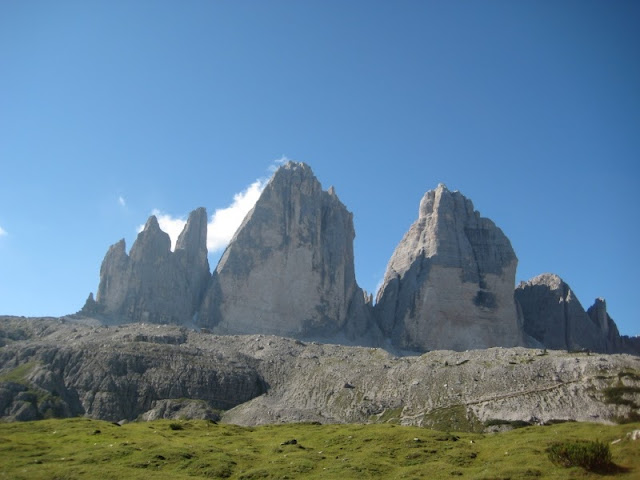
\includegraphics[width=.9\textwidth]{images/drei_zinnen.jpg}
\end{figure}
\end{column}
\end{columns}
\end{frame}

\appendix
\pagenumbering{Roman}

%%%%%%%%%%%%%%%%%%%%%%%%%%%%%%%%% Appendix %%%%%%%%%%%%%%%%%%%%%%%%%%%%%%%%%%%%%%%%%%

\section{Bibliography}
\begin{frame}[allowframebreaks]{Literature}
\bibliographystyle{unsrt}
\bibliography{../latex/bibtex/Master_Thesis,../latex/bibtex/manual}
\end{frame}

%\section{Additional Material}
%\begin{frame}{Use Case Overview}
%\begin{figure}
%    \centering
%    \includegraphics[height=0.7\textheight]{../latex/diagrams/use_cases_overall.pdf}
%    \caption{Overall use case diagram (UML use case diagram)}
%\end{figure}
%\end{frame}

%\begin{frame}[allowframebreaks]{Object Design}
%\begin{figure}
%    \centering
%    \includegraphics[height=0.5\textheight]{../latex/diagrams/InteractionPatterns.pdf}
%    \caption{Matching Interactions to InteractionPatterns (UML class diagram)}
%\end{figure}

\end{document}
